\documentclass{article}
\usepackage{graphicx} % Required for inserting images
\usepackage{mathtools}
\usepackage{xcolor}
\usepackage{subcaption}
\title{Implementation}
\author{Group 5}
\date{November 2023}

\begin{document}

\maketitle

\section{Problem Presentation}

\noindent The FEM method is used to modelize and resolve a real physics problem, our goal is to find the deflection vector $u(x)$.
We have modelized the problem and it consists into a linear problem of the form: $A\cdot \Vec{u}=\Vec{b}$.
\begin{enumerate}
\item 
Our job is to implement in Julia programming language a function that solves the linear system.
Julia provides an easy solution to that problem: the "\textbackslash" operator. So we implemented a Type safe function that takes the matrix $A$ and the vector $\Vec{b}$ with floating values, and returns the vector $\Vec{u}$ as a float. To control the type-safety of the function we used the macro \textcolor{magenta}{$@code \textunderscore warntype$}.
\newpage
\item 
Our second job was to compare the time complexity required to solve linear problem in which the $A$ matrix changed its form using the \textcolor{magenta}{$@elapsed$} macro:
firstly we have considered a matrix stored in memory as a sparse matrix and then as a full matrix. To build the Matrixes we used the function $sprand$ that randomize the position of the numbers given a density and the dimension of the matrix. To generate the dense function, which has the zero in place of points, we used the function: $Matrix$ which takes the sparse matrix and denses it We saw that the "\textbackslash" operator is faster with the full one:
\begin{figure}[h]
    \centering
    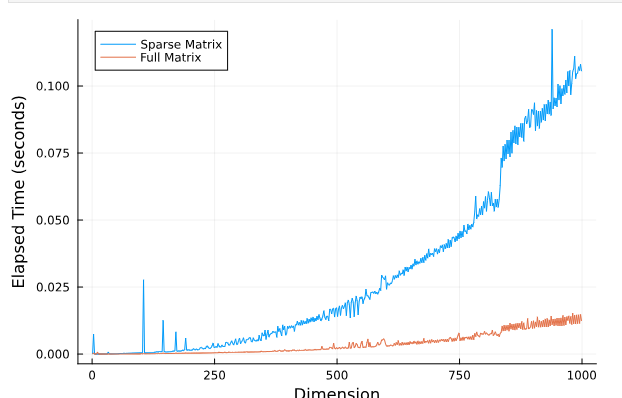
\includegraphics[width=0.7\linewidth]{sparsevsfull.png}
    \caption{This is a graphic of elapsed time of solving the problem in base of the dimension of the matrix}
    \label{fig:enter-label}
\end{figure}

\item {
Considering the second point conclusion, we have generated a tridiagonal matrix in Julia and compared how the operator worked on tridiagonal matrixes and tridiagonal full matrixes. We came to the conclusion that is way better to store the matrix as a tridiagonal because storing zeros leads to overhead:

    \begin{figure}[h]
      \centering
      \begin{subfigure}[b]{0.75\textwidth}
        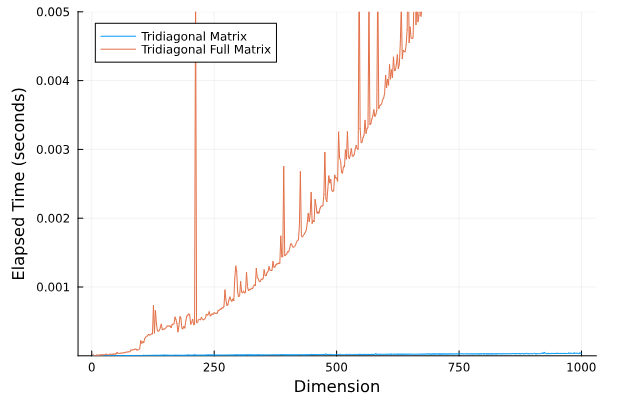
\includegraphics[width=\textwidth]{tridiagonal1.png} % Replace with your first image
        \caption{Zoomed out}
        \label{fig:subfig1}
      \end{subfigure}
      \hfill
      \begin{subfigure}[b]{0.75\textwidth}
        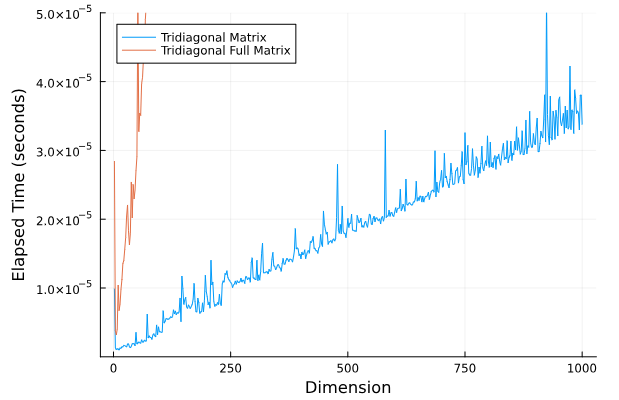
\includegraphics[width=\textwidth]{tridiagonal2.png} % Replace with your second image
        \caption{Zoomed in}
        \label{fig:subfig2}
      \end{subfigure}
      \caption{Two different perspectives of the elapsed time for the tridiagonal matrixes}
      \label{fig:mainfig}
    \end{figure}
}
\end{enumerate}


\end{document}
